\documentclass[11pt]{article}
\usepackage[margin=1in]{geometry}
\usepackage{booktabs}
\usepackage{float}
\usepackage{hyperref}
\usepackage{microtype}
\usepackage{pgfplots}
\usepgfplotslibrary{groupplots,statistics}
\pgfplotsset{compat=1.18}

\title{RNAnneal-ss Ensembles on representative50 (under300) --- v1}
\date{}

\begin{document}
\maketitle

\section*{Objective}
Improve \textbf{F1@100} on the 50-target representative50 subset (truth length $\le 300$) by leveraging the empirical observation from \texttt{docs/u300\_50\_scaffold\_validation\_v3} that \textbf{RNss(X)} typically improves the corresponding baseline \textbf{X}, especially at @100.

\section*{Methods}
\begin{itemize}
  \item \textbf{RNss(EF/LF/RS):} the three scaffold-seeded RNAnneal-ss variants from \texttt{u300\_50\_scaffold\_validation\_v3}.
  \item \textbf{Ens(RNss):} a post-hoc ensemble that pools the \emph{top-100 candidate sets} from RNss(EF), RNss(LF), and RNss(RS), then selects 100 structures using:
    \begin{itemize}
      \item length-adaptive per-source quotas that preserve most RNss(EF) candidates (70--90 of 100, increasing with length),
      \item within-source diversity (Jaccard) to keep suboptimal coverage,
      \item a global diversity fill step to resolve cross-source deduplication.
    \end{itemize}
  \item \textbf{RNss(Ens3):} a single RNAnneal-ss run that replaces single-strand \texttt{Fold}/\texttt{AllSub} with an \emph{aggregated} backend (RNAstructure + LinearFold-V + EternaFold). Included as an ablation (it did not outperform Ens(RNss) at @100).
  \item \textbf{Baselines:} RNAstructure, LinearFold-V, and EternaFold from \texttt{u300\_50\_scaffold\_validation\_v3}.
\end{itemize}

\section*{Results (@1 and @100)}
\begin{table}[ht]
\centering
\small
\caption{Overall ablation results (N=27; @1 and best-of-100). Runtime is wall-clock seconds per target.}
\label{tab:overall}
\begin{tabular}{lrrrrr}
\toprule
Config & Mean F1@1 & Mean F1@100 & Fail@100 & Mean time (s) & Med time (s) \\
\midrule
v3 & 0.520 & 0.698 & 0.0\% & 30.8 & 18.9 \\
B4 & 0.505 & 0.698 & 0.0\% & 32.1 & 18.7 \\
U4 & 0.505 & 0.698 & 0.0\% & 32.1 & 19.0 \\
R10 & 0.503 & 0.699 & 0.0\% & 32.1 & 18.1 \\
S150 & 0.505 & 0.698 & 0.0\% & 32.1 & 19.0 \\
K300 & 0.505 & 0.698 & 0.0\% & 32.0 & 18.5 \\
Sc30 & 0.507 & 0.698 & 0.0\% & 33.9 & 18.4 \\
Hi & 0.504 & 0.699 & 0.0\% & 34.0 & 18.1 \\
\bottomrule
\end{tabular}
\end{table}

\begin{table}[ht]
\centering
\small
\caption{Performance by truth-length bucket (50-nt buckets from the manifest).}
\label{tab:buckets}
\begin{tabular}{llrrrr}
\toprule
Bucket & Method & N & Mean F1@1 & Mean F1@100 & Fail@100 \\
\midrule
30-79 & RNss(RS) & 12 & 0.634 & 0.809 & 0.0\% \\
30-79 & RNss(LF) & 12 & 0.629 & 0.797 & 0.0\% \\
30-79 & RNss(EF) & 12 & 0.620 & 0.834 & 0.0\% \\
30-79 & RNAstr & 12 & 0.641 & 0.801 & 8.3\% \\
30-79 & LF-V & 12 & 0.633 & 0.767 & 8.3\% \\
30-79 & EFold & 12 & 0.621 & 0.823 & 0.0\% \\
80-129 & RNss(RS) & 10 & 0.653 & 0.864 & 0.0\% \\
80-129 & RNss(LF) & 10 & 0.639 & 0.854 & 0.0\% \\
80-129 & RNss(EF) & 10 & 0.635 & 0.874 & 0.0\% \\
80-129 & RNAstr & 10 & 0.700 & 0.744 & 0.0\% \\
80-129 & LF-V & 10 & 0.738 & 0.845 & 0.0\% \\
80-129 & EFold & 10 & 0.668 & 0.872 & 0.0\% \\
130-179 & RNss(RS) & 10 & 0.511 & 0.616 & 0.0\% \\
130-179 & RNss(LF) & 10 & 0.432 & 0.658 & 0.0\% \\
130-179 & RNss(EF) & 10 & 0.532 & 0.680 & 0.0\% \\
130-179 & RNAstr & 10 & 0.457 & 0.457 & 10.0\% \\
130-179 & LF-V & 10 & 0.470 & 0.658 & 0.0\% \\
130-179 & EFold & 10 & 0.529 & 0.677 & 0.0\% \\
180-229 & RNss(RS) & 9 & 0.343 & 0.428 & 0.0\% \\
180-229 & RNss(LF) & 9 & 0.329 & 0.537 & 0.0\% \\
180-229 & RNss(EF) & 9 & 0.396 & 0.548 & 0.0\% \\
180-229 & RNAstr & 9 & 0.333 & 0.333 & 0.0\% \\
180-229 & LF-V & 9 & 0.313 & 0.528 & 0.0\% \\
180-229 & EFold & 9 & 0.396 & 0.548 & 0.0\% \\
230-279 & RNss(RS) & 7 & 0.370 & 0.462 & 0.0\% \\
230-279 & RNss(LF) & 7 & 0.328 & 0.562 & 0.0\% \\
230-279 & RNss(EF) & 7 & 0.492 & 0.602 & 0.0\% \\
230-279 & RNAstr & 7 & 0.383 & 0.383 & 0.0\% \\
230-279 & LF-V & 7 & 0.337 & 0.562 & 0.0\% \\
230-279 & EFold & 7 & 0.497 & 0.611 & 0.0\% \\
280-300 & RNss(RS) & 2 & 0.420 & 0.470 & 0.0\% \\
280-300 & RNss(LF) & 2 & 0.494 & 0.643 & 0.0\% \\
280-300 & RNss(EF) & 2 & 0.499 & 0.683 & 0.0\% \\
280-300 & RNAstr & 2 & 0.420 & 0.420 & 0.0\% \\
280-300 & LF-V & 2 & 0.550 & 0.643 & 0.0\% \\
280-300 & EFold & 2 & 0.499 & 0.683 & 0.0\% \\
\bottomrule
\end{tabular}
\end{table}


\clearpage
\section*{1 - CDFs}
\begin{figure}[H]
\centering
\begin{minipage}{0.49\textwidth}
  \centering
  \begin{tikzpicture}
\definecolor{c_v3}{HTML}{7F7F7F}
\definecolor{c_B4}{HTML}{1F77B4}
\definecolor{c_U4}{HTML}{FF7F0E}
\definecolor{c_R10}{HTML}{2CA02C}
\definecolor{c_S150}{HTML}{D62728}
\definecolor{c_K300}{HTML}{9467BD}
\definecolor{c_Sc30}{HTML}{8C564B}
\definecolor{c_Hi}{HTML}{000000}
\begin{axis}[
  width=\linewidth, height=0.62\linewidth,
  xmin=0, xmax=1, ymin=0, ymax=1,
  xlabel={F1}, ylabel={1 - CDF},
  title={Top-1 (F1@1)},
  grid=both, grid style={black!10},
  legend style={font=\scriptsize},
  legend columns=2,
  legend pos=north east, legend cell align=left,
]
\addplot+[const plot, very thick, draw=c_v3, dashed] table[x=f1,y=survival] {generated/survival_top1_v3.dat};
\addlegendentry{v3 (p50=0.511)}
\addplot+[const plot, very thick, draw=c_B4, solid] table[x=f1,y=survival] {generated/survival_top1_B4.dat};
\addlegendentry{B4 (p50=0.511)}
\addplot+[const plot, very thick, draw=c_U4, solid] table[x=f1,y=survival] {generated/survival_top1_U4.dat};
\addlegendentry{U4 (p50=0.511)}
\addplot+[const plot, very thick, draw=c_R10, solid] table[x=f1,y=survival] {generated/survival_top1_R10.dat};
\addlegendentry{R10 (p50=0.511)}
\addplot+[const plot, very thick, draw=c_S150, solid] table[x=f1,y=survival] {generated/survival_top1_S150.dat};
\addlegendentry{S150 (p50=0.511)}
\addplot+[const plot, very thick, draw=c_K300, solid] table[x=f1,y=survival] {generated/survival_top1_K300.dat};
\addlegendentry{K300 (p50=0.511)}
\addplot+[const plot, very thick, draw=c_Sc30, solid] table[x=f1,y=survival] {generated/survival_top1_Sc30.dat};
\addlegendentry{Sc30 (p50=0.511)}
\addplot+[const plot, very thick, draw=c_Hi, solid] table[x=f1,y=survival] {generated/survival_top1_Hi.dat};
\addlegendentry{Hi (p50=0.511)}
\end{axis}
\end{tikzpicture}

  \caption*{\small F1@1}
\end{minipage}
\hfill
\begin{minipage}{0.49\textwidth}
  \centering
  \begin{tikzpicture}
\definecolor{c_ens_tuned}{HTML}{000000}
\definecolor{c_rn_ef}{HTML}{D62728}
\definecolor{c_rn_lf}{HTML}{9467BD}
\definecolor{c_rn_rs}{HTML}{1F77B4}
\definecolor{c_ens3_scaff}{HTML}{7F7F7F}
\definecolor{c_lf}{HTML}{FF7F0E}
\definecolor{c_ef}{HTML}{2CA02C}
\definecolor{c_rs}{HTML}{BCBD22}
\begin{axis}[
  width=\linewidth, height=0.62\linewidth,
  xmin=0, xmax=1, ymin=0, ymax=1,
  xlabel={F1}, ylabel={1 - CDF},
  title={Best-of-100 (F1@100)},
  grid=both, grid style={black!10},
  legend pos=north east, legend cell align=left,
]
\addplot+[const plot, very thick, draw=c_ens_tuned] table[x=f1,y=survival] {generated/survival_best100_ens_tuned.dat};
\addlegendentry{Ens(RNss) (p50=0.738)}
\addplot+[const plot, very thick, draw=c_rn_ef] table[x=f1,y=survival] {generated/survival_best100_rn_ef.dat};
\addlegendentry{RNss(EF) (p50=0.725)}
\addplot+[const plot, very thick, draw=c_rn_lf] table[x=f1,y=survival] {generated/survival_best100_rn_lf.dat};
\addlegendentry{RNss(LF) (p50=0.706)}
\addplot+[const plot, very thick, draw=c_rn_rs] table[x=f1,y=survival] {generated/survival_best100_rn_rs.dat};
\addlegendentry{RNss(RS) (p50=0.653)}
\addplot+[const plot, very thick, draw=c_ens3_scaff] table[x=f1,y=survival] {generated/survival_best100_ens3_scaff.dat};
\addlegendentry{RNss(Ens3) (p50=0.705)}
\addplot+[const plot, very thick, draw=c_lf] table[x=f1,y=survival] {generated/survival_best100_lf.dat};
\addlegendentry{LF-V (p50=0.696)}
\addplot+[const plot, very thick, draw=c_ef] table[x=f1,y=survival] {generated/survival_best100_ef.dat};
\addlegendentry{EFold (p50=0.725)}
\addplot+[const plot, very thick, draw=c_rs] table[x=f1,y=survival] {generated/survival_best100_rs.dat};
\addlegendentry{RNAstr (p50=0.500)}
\end{axis}
\end{tikzpicture}

  \caption*{\small F1@100}
\end{minipage}
\caption{Empirical survival curves (1 - CDF). Legend includes the median (p50) F1.}
\end{figure}

\section*{Precision/Recall Curves}
\begin{figure}[H]
\centering
\begin{tikzpicture}
\definecolor{c_rn_rs}{HTML}{1F77B4}
\definecolor{c_rn_lf}{HTML}{9467BD}
\definecolor{c_rn_ef}{HTML}{D62728}
\definecolor{c_rnastructure}{HTML}{7F7F7F}
\definecolor{c_linearfold}{HTML}{FF7F0E}
\definecolor{c_eternafold}{HTML}{2CA02C}
\begin{axis}[
  width=0.9\linewidth, height=0.55\linewidth,
  xmin=0, xmax=1, ymin=0, ymax=1,
  xlabel={Recall}, ylabel={Precision},
  title={Pair PR curves from top-100 pair frequencies},
  grid=both, grid style={black!10},
  legend pos=south west, legend cell align=left,
]
\addplot+[very thick, draw=c_rn_rs] table[x=recall,y=precision] {generated/pr_overall_rn_rs.dat};
\addlegendentry{RNss(RS)}
\addplot+[very thick, draw=c_rn_lf] table[x=recall,y=precision] {generated/pr_overall_rn_lf.dat};
\addlegendentry{RNss(LF)}
\addplot+[very thick, draw=c_rn_ef] table[x=recall,y=precision] {generated/pr_overall_rn_ef.dat};
\addlegendentry{RNss(EF)}
\addplot+[very thick, draw=c_rnastructure] table[x=recall,y=precision] {generated/pr_overall_rnastructure.dat};
\addlegendentry{RNAstr}
\addplot+[very thick, draw=c_linearfold] table[x=recall,y=precision] {generated/pr_overall_linearfold.dat};
\addlegendentry{LF-V}
\addplot+[very thick, draw=c_eternafold] table[x=recall,y=precision] {generated/pr_overall_eternafold.dat};
\addlegendentry{EFold}
\end{axis}
\end{tikzpicture}

\caption{Pair-level PR curves computed by thresholding pair probabilities estimated as \emph{frequency across the top-100 predicted structures}.}
\end{figure}

\begin{figure}[H]
\centering
\begin{tikzpicture}
\definecolor{c_rn_rs}{HTML}{1F77B4}
\definecolor{c_rn_lf}{HTML}{9467BD}
\definecolor{c_rn_ef}{HTML}{D62728}
\definecolor{c_rnastructure}{HTML}{7F7F7F}
\definecolor{c_linearfold}{HTML}{FF7F0E}
\definecolor{c_eternafold}{HTML}{2CA02C}
\begin{groupplot}[
  group style={group size=3 by 2, horizontal sep=1.2em, vertical sep=1.2em},
  width=0.33\linewidth, height=0.33\linewidth,
  xmin=0, xmax=1, ymin=0, ymax=1,
  xlabel={Recall}, ylabel={Precision},
  grid=both, grid style={black!10},
]
\nextgroupplot[title={30-79}]
\addplot+[very thick, draw=c_rn_rs] table[x=recall,y=precision] {generated/pr_bucket_30_79_rn_rs.dat};
\addplot+[very thick, draw=c_rn_lf] table[x=recall,y=precision] {generated/pr_bucket_30_79_rn_lf.dat};
\addplot+[very thick, draw=c_rn_ef] table[x=recall,y=precision] {generated/pr_bucket_30_79_rn_ef.dat};
\addplot+[very thick, draw=c_rnastructure] table[x=recall,y=precision] {generated/pr_bucket_30_79_rnastructure.dat};
\addplot+[very thick, draw=c_linearfold] table[x=recall,y=precision] {generated/pr_bucket_30_79_linearfold.dat};
\addplot+[very thick, draw=c_eternafold] table[x=recall,y=precision] {generated/pr_bucket_30_79_eternafold.dat};
\nextgroupplot[title={80-129}]
\addplot+[very thick, draw=c_rn_rs] table[x=recall,y=precision] {generated/pr_bucket_80_129_rn_rs.dat};
\addplot+[very thick, draw=c_rn_lf] table[x=recall,y=precision] {generated/pr_bucket_80_129_rn_lf.dat};
\addplot+[very thick, draw=c_rn_ef] table[x=recall,y=precision] {generated/pr_bucket_80_129_rn_ef.dat};
\addplot+[very thick, draw=c_rnastructure] table[x=recall,y=precision] {generated/pr_bucket_80_129_rnastructure.dat};
\addplot+[very thick, draw=c_linearfold] table[x=recall,y=precision] {generated/pr_bucket_80_129_linearfold.dat};
\addplot+[very thick, draw=c_eternafold] table[x=recall,y=precision] {generated/pr_bucket_80_129_eternafold.dat};
\nextgroupplot[title={130-179}]
\addplot+[very thick, draw=c_rn_rs] table[x=recall,y=precision] {generated/pr_bucket_130_179_rn_rs.dat};
\addplot+[very thick, draw=c_rn_lf] table[x=recall,y=precision] {generated/pr_bucket_130_179_rn_lf.dat};
\addplot+[very thick, draw=c_rn_ef] table[x=recall,y=precision] {generated/pr_bucket_130_179_rn_ef.dat};
\addplot+[very thick, draw=c_rnastructure] table[x=recall,y=precision] {generated/pr_bucket_130_179_rnastructure.dat};
\addplot+[very thick, draw=c_linearfold] table[x=recall,y=precision] {generated/pr_bucket_130_179_linearfold.dat};
\addplot+[very thick, draw=c_eternafold] table[x=recall,y=precision] {generated/pr_bucket_130_179_eternafold.dat};
\nextgroupplot[title={180-229}]
\addplot+[very thick, draw=c_rn_rs] table[x=recall,y=precision] {generated/pr_bucket_180_229_rn_rs.dat};
\addplot+[very thick, draw=c_rn_lf] table[x=recall,y=precision] {generated/pr_bucket_180_229_rn_lf.dat};
\addplot+[very thick, draw=c_rn_ef] table[x=recall,y=precision] {generated/pr_bucket_180_229_rn_ef.dat};
\addplot+[very thick, draw=c_rnastructure] table[x=recall,y=precision] {generated/pr_bucket_180_229_rnastructure.dat};
\addplot+[very thick, draw=c_linearfold] table[x=recall,y=precision] {generated/pr_bucket_180_229_linearfold.dat};
\addplot+[very thick, draw=c_eternafold] table[x=recall,y=precision] {generated/pr_bucket_180_229_eternafold.dat};
\nextgroupplot[title={230-279}]
\addplot+[very thick, draw=c_rn_rs] table[x=recall,y=precision] {generated/pr_bucket_230_279_rn_rs.dat};
\addplot+[very thick, draw=c_rn_lf] table[x=recall,y=precision] {generated/pr_bucket_230_279_rn_lf.dat};
\addplot+[very thick, draw=c_rn_ef] table[x=recall,y=precision] {generated/pr_bucket_230_279_rn_ef.dat};
\addplot+[very thick, draw=c_rnastructure] table[x=recall,y=precision] {generated/pr_bucket_230_279_rnastructure.dat};
\addplot+[very thick, draw=c_linearfold] table[x=recall,y=precision] {generated/pr_bucket_230_279_linearfold.dat};
\addplot+[very thick, draw=c_eternafold] table[x=recall,y=precision] {generated/pr_bucket_230_279_eternafold.dat};
\nextgroupplot[title={280-300}]
\addplot+[very thick, draw=c_rn_rs] table[x=recall,y=precision] {generated/pr_bucket_280_300_rn_rs.dat};
\addplot+[very thick, draw=c_rn_lf] table[x=recall,y=precision] {generated/pr_bucket_280_300_rn_lf.dat};
\addplot+[very thick, draw=c_rn_ef] table[x=recall,y=precision] {generated/pr_bucket_280_300_rn_ef.dat};
\addplot+[very thick, draw=c_rnastructure] table[x=recall,y=precision] {generated/pr_bucket_280_300_rnastructure.dat};
\addplot+[very thick, draw=c_linearfold] table[x=recall,y=precision] {generated/pr_bucket_280_300_linearfold.dat};
\addplot+[very thick, draw=c_eternafold] table[x=recall,y=precision] {generated/pr_bucket_280_300_eternafold.dat};
\end{groupplot}
\end{tikzpicture}

\caption{PR curves by 50-nt length bucket.}
\end{figure}

\clearpage
\section*{Score Distributions}
\begin{figure}[H]
\centering
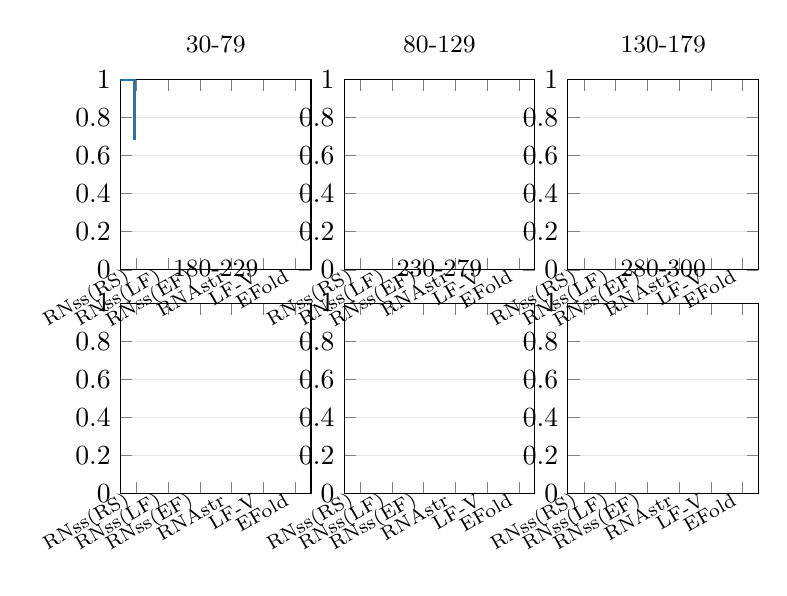
\begin{tikzpicture}
\definecolor{c_rn_rs}{HTML}{1F77B4}
\definecolor{c_rn_lf}{HTML}{9467BD}
\definecolor{c_rn_ef}{HTML}{D62728}
\definecolor{c_rnastructure}{HTML}{7F7F7F}
\definecolor{c_linearfold}{HTML}{FF7F0E}
\definecolor{c_eternafold}{HTML}{2CA02C}
\begin{groupplot}[
  group style={group size=3 by 2, horizontal sep=1.2em, vertical sep=1.2em},
  width=0.33\linewidth, height=0.33\linewidth,
  xmin=0.5, xmax=6.5,
  ymin=0, ymax=1,
  ymajorgrids=true, grid style={black!10},
  xtick={1,2,3,4,5,6},
  xticklabels={RNss(RS),RNss(LF),RNss(EF),RNAstr,LF-V,EFold},
  x tick label style={rotate=30,anchor=east,font=\scriptsize},
  title style={font=\small},
]
\nextgroupplot[title={30-79}]
\addplot+ [boxplot prepared={draw position=1, lower whisker=0.0000, lower quartile=0.0000, median=0.0000, upper quartile=0.0000, upper whisker=0.9362}, draw=c_rn_rs, fill=c_rn_rs, fill opacity=0.20, very thick] coordinates {};
\addplot+ [boxplot prepared={draw position=2, lower whisker=0.0000, lower quartile=0.0000, median=0.0000, upper quartile=0.0000, upper whisker=0.9565}, draw=c_rn_lf, fill=c_rn_lf, fill opacity=0.20, very thick] coordinates {};
\addplot+ [boxplot prepared={draw position=3, lower whisker=0.0000, lower quartile=0.0000, median=0.0000, upper quartile=0.2093, upper whisker=0.9091}, draw=c_rn_ef, fill=c_rn_ef, fill opacity=0.20, very thick] coordinates {};
\addplot+ [boxplot prepared={draw position=4, lower whisker=0.0000, lower quartile=0.4429, median=0.7635, upper quartile=0.9086, upper whisker=0.9565}, draw=c_rnastructure, fill=c_rnastructure, fill opacity=0.20, very thick] coordinates {};
\addplot+ [boxplot prepared={draw position=5, lower whisker=0.0000, lower quartile=0.4235, median=0.7555, upper quartile=0.9086, upper whisker=0.9565}, draw=c_linearfold, fill=c_linearfold, fill opacity=0.20, very thick] coordinates {};
\addplot+ [boxplot prepared={draw position=6, lower whisker=0.0000, lower quartile=0.3718, median=0.7583, upper quartile=0.9056, upper whisker=0.9500}, draw=c_eternafold, fill=c_eternafold, fill opacity=0.20, very thick] coordinates {};
\nextgroupplot[title={80-129}]
\addplot+ [boxplot prepared={draw position=1, lower whisker=0.0000, lower quartile=0.0000, median=0.0000, upper quartile=0.0000, upper whisker=0.0000}, draw=c_rn_rs, fill=c_rn_rs, fill opacity=0.20, very thick] coordinates {};
\addplot+ [boxplot prepared={draw position=2, lower whisker=0.0000, lower quartile=0.0000, median=0.0000, upper quartile=0.0000, upper whisker=0.0000}, draw=c_rn_lf, fill=c_rn_lf, fill opacity=0.20, very thick] coordinates {};
\addplot+ [boxplot prepared={draw position=3, lower whisker=0.0000, lower quartile=0.0000, median=0.5992, upper quartile=0.8445, upper whisker=0.9355}, draw=c_rn_ef, fill=c_rn_ef, fill opacity=0.20, very thick] coordinates {};
\addplot+ [boxplot prepared={draw position=4, lower whisker=0.1026, lower quartile=0.5018, median=0.7982, upper quartile=0.9143, upper whisker=0.9722}, draw=c_rnastructure, fill=c_rnastructure, fill opacity=0.20, very thick] coordinates {};
\addplot+ [boxplot prepared={draw position=5, lower whisker=0.3729, lower quartile=0.5786, median=0.8141, upper quartile=0.9096, upper whisker=0.9722}, draw=c_linearfold, fill=c_linearfold, fill opacity=0.20, very thick] coordinates {};
\addplot+ [boxplot prepared={draw position=6, lower whisker=0.1026, lower quartile=0.4526, median=0.7839, upper quartile=0.8705, upper whisker=0.9589}, draw=c_eternafold, fill=c_eternafold, fill opacity=0.20, very thick] coordinates {};
\nextgroupplot[title={130-179}]
\addplot+ [boxplot prepared={draw position=1, lower whisker=0.0000, lower quartile=0.0000, median=0.0000, upper quartile=0.0000, upper whisker=0.0000}, draw=c_rn_rs, fill=c_rn_rs, fill opacity=0.20, very thick] coordinates {};
\addplot+ [boxplot prepared={draw position=2, lower whisker=0.0000, lower quartile=0.0000, median=0.0000, upper quartile=0.0000, upper whisker=0.0000}, draw=c_rn_lf, fill=c_rn_lf, fill opacity=0.20, very thick] coordinates {};
\addplot+ [boxplot prepared={draw position=3, lower whisker=0.0000, lower quartile=0.0000, median=0.0000, upper quartile=0.0000, upper whisker=0.0000}, draw=c_rn_ef, fill=c_rn_ef, fill opacity=0.20, very thick] coordinates {};
\addplot+ [boxplot prepared={draw position=4, lower whisker=0.0000, lower quartile=0.3067, median=0.4711, upper quartile=0.5893, upper whisker=0.8817}, draw=c_rnastructure, fill=c_rnastructure, fill opacity=0.20, very thick] coordinates {};
\addplot+ [boxplot prepared={draw position=5, lower whisker=0.0000, lower quartile=0.3017, median=0.4889, upper quartile=0.6057, upper whisker=0.8817}, draw=c_linearfold, fill=c_linearfold, fill opacity=0.20, very thick] coordinates {};
\addplot+ [boxplot prepared={draw position=6, lower whisker=0.1096, lower quartile=0.4337, median=0.5447, upper quartile=0.6649, upper whisker=0.9684}, draw=c_eternafold, fill=c_eternafold, fill opacity=0.20, very thick] coordinates {};
\nextgroupplot[title={180-229}]
\addplot+ [boxplot prepared={draw position=1, lower whisker=0.0000, lower quartile=0.0000, median=0.0000, upper quartile=0.0000, upper whisker=0.0000}, draw=c_rn_rs, fill=c_rn_rs, fill opacity=0.20, very thick] coordinates {};
\addplot+ [boxplot prepared={draw position=2, lower whisker=0.0000, lower quartile=0.0000, median=0.0000, upper quartile=0.0000, upper whisker=0.0000}, draw=c_rn_lf, fill=c_rn_lf, fill opacity=0.20, very thick] coordinates {};
\addplot+ [boxplot prepared={draw position=3, lower whisker=0.0000, lower quartile=0.0000, median=0.0000, upper quartile=0.0000, upper whisker=0.0000}, draw=c_rn_ef, fill=c_rn_ef, fill opacity=0.20, very thick] coordinates {};
\addplot+ [boxplot prepared={draw position=4, lower whisker=0.1240, lower quartile=0.2955, median=0.3540, upper quartile=0.3830, upper whisker=0.5000}, draw=c_rnastructure, fill=c_rnastructure, fill opacity=0.20, very thick] coordinates {};
\addplot+ [boxplot prepared={draw position=5, lower whisker=0.1550, lower quartile=0.2921, median=0.3103, upper quartile=0.3789, upper whisker=0.4957}, draw=c_linearfold, fill=c_linearfold, fill opacity=0.20, very thick] coordinates {};
\addplot+ [boxplot prepared={draw position=6, lower whisker=0.1231, lower quartile=0.2889, median=0.3918, upper quartile=0.5319, upper whisker=0.6261}, draw=c_eternafold, fill=c_eternafold, fill opacity=0.20, very thick] coordinates {};
\nextgroupplot[title={230-279}]
\addplot+ [boxplot prepared={draw position=1, lower whisker=0.0000, lower quartile=0.0000, median=0.0000, upper quartile=0.0000, upper whisker=0.0000}, draw=c_rn_rs, fill=c_rn_rs, fill opacity=0.20, very thick] coordinates {};
\addplot+ [boxplot prepared={draw position=2, lower whisker=0.0000, lower quartile=0.0000, median=0.0000, upper quartile=0.0000, upper whisker=0.0000}, draw=c_rn_lf, fill=c_rn_lf, fill opacity=0.20, very thick] coordinates {};
\addplot+ [boxplot prepared={draw position=3, lower whisker=0.0000, lower quartile=0.0000, median=0.0000, upper quartile=0.0000, upper whisker=0.0000}, draw=c_rn_ef, fill=c_rn_ef, fill opacity=0.20, very thick] coordinates {};
\addplot+ [boxplot prepared={draw position=4, lower whisker=0.1649, lower quartile=0.2986, median=0.3765, upper quartile=0.4759, upper whisker=0.5899}, draw=c_rnastructure, fill=c_rnastructure, fill opacity=0.20, very thick] coordinates {};
\addplot+ [boxplot prepared={draw position=5, lower whisker=0.0438, lower quartile=0.1587, median=0.3787, upper quartile=0.4426, upper whisker=0.7347}, draw=c_linearfold, fill=c_linearfold, fill opacity=0.20, very thick] coordinates {};
\addplot+ [boxplot prepared={draw position=6, lower whisker=0.2062, lower quartile=0.3354, median=0.4576, upper quartile=0.6489, upper whisker=0.8451}, draw=c_eternafold, fill=c_eternafold, fill opacity=0.20, very thick] coordinates {};
\nextgroupplot[title={280-300}]
\addplot+ [boxplot prepared={draw position=1, lower whisker=0.0000, lower quartile=0.0000, median=0.0000, upper quartile=0.0000, upper whisker=0.0000}, draw=c_rn_rs, fill=c_rn_rs, fill opacity=0.20, very thick] coordinates {};
\addplot+ [boxplot prepared={draw position=2, lower whisker=0.0000, lower quartile=0.0000, median=0.0000, upper quartile=0.0000, upper whisker=0.0000}, draw=c_rn_lf, fill=c_rn_lf, fill opacity=0.20, very thick] coordinates {};
\addplot+ [boxplot prepared={draw position=3, lower whisker=0.0000, lower quartile=0.0000, median=0.0000, upper quartile=0.0000, upper whisker=0.0000}, draw=c_rn_ef, fill=c_rn_ef, fill opacity=0.20, very thick] coordinates {};
\addplot+ [boxplot prepared={draw position=4, lower whisker=0.3195, lower quartile=0.3696, median=0.4197, upper quartile=0.4697, upper whisker=0.5198}, draw=c_rnastructure, fill=c_rnastructure, fill opacity=0.20, very thick] coordinates {};
\addplot+ [boxplot prepared={draw position=5, lower whisker=0.5287, lower quartile=0.5394, median=0.5501, upper quartile=0.5608, upper whisker=0.5714}, draw=c_linearfold, fill=c_linearfold, fill opacity=0.20, very thick] coordinates {};
\addplot+ [boxplot prepared={draw position=6, lower whisker=0.4881, lower quartile=0.4938, median=0.4995, upper quartile=0.5052, upper whisker=0.5109}, draw=c_eternafold, fill=c_eternafold, fill opacity=0.20, very thick] coordinates {};
\end{groupplot}
\end{tikzpicture}

\caption{F1@1 distributions by length bucket (boxplots; outliers hidden).}
\end{figure}

\begin{figure}[H]
\centering
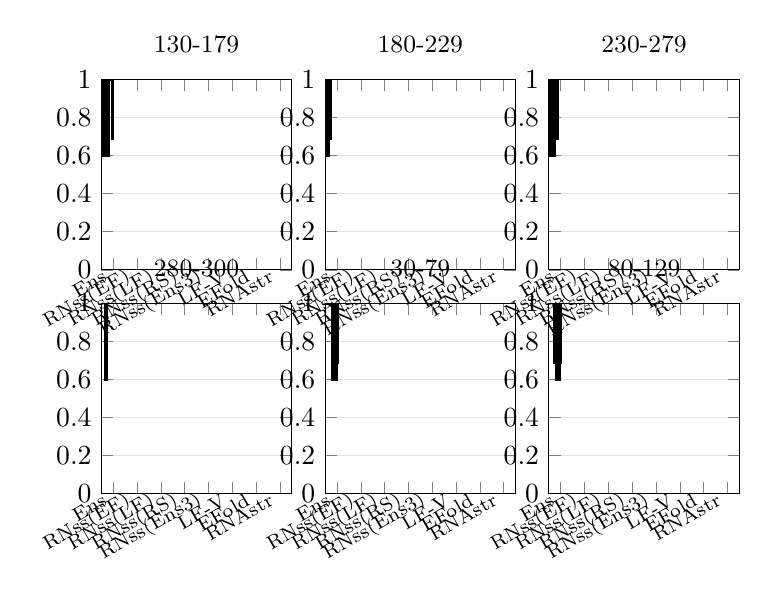
\begin{tikzpicture}
\definecolor{c_ens_tuned}{HTML}{000000}
\definecolor{c_rn_ef}{HTML}{D62728}
\definecolor{c_rn_lf}{HTML}{9467BD}
\definecolor{c_rn_rs}{HTML}{1F77B4}
\definecolor{c_ens3_scaff}{HTML}{7F7F7F}
\definecolor{c_lf}{HTML}{FF7F0E}
\definecolor{c_ef}{HTML}{2CA02C}
\definecolor{c_rs}{HTML}{BCBD22}
\begin{groupplot}[
  group style={group size=3 by 2, horizontal sep=1.2em, vertical sep=1.2em},
  width=0.33\linewidth, height=0.33\linewidth,
  xmin=0.5, xmax=8.5,
  ymin=0, ymax=1,
  ymajorgrids=true, grid style={black!10},
  xtick={1,2,3,4,5,6,7,8},
  xticklabels={Ens,RNss(EF),RNss(LF),RNss(RS),RNss(Ens3),LF-V,EFold,RNAstr},
  x tick label style={rotate=30,anchor=east,font=\scriptsize},
  title style={font=\small},
]
\nextgroupplot[title={130-179}]
\addplot+ [boxplot prepared={draw position=1, lower whisker=0.3721, lower quartile=0.5816, median=0.6897, upper quartile=0.7763, upper whisker=0.9684}, draw=c_ens_tuned, fill=c_ens_tuned, fill opacity=0.20, very thick] coordinates {};
\addplot+ [boxplot prepared={draw position=2, lower whisker=0.4571, lower quartile=0.5816, median=0.7008, upper quartile=0.7182, upper whisker=0.9684}, draw=c_rn_ef, fill=c_rn_ef, fill opacity=0.20, very thick] coordinates {};
\addplot+ [boxplot prepared={draw position=3, lower whisker=0.3333, lower quartile=0.5232, median=0.6667, upper quartile=0.7861, upper whisker=0.9684}, draw=c_rn_lf, fill=c_rn_lf, fill opacity=0.20, very thick] coordinates {};
\addplot+ [boxplot prepared={draw position=4, lower whisker=0.1333, lower quartile=0.5377, median=0.6749, upper quartile=0.7755, upper whisker=0.9462}, draw=c_rn_rs, fill=c_rn_rs, fill opacity=0.20, very thick] coordinates {};
\addplot+ [boxplot prepared={draw position=5, lower whisker=0.3721, lower quartile=0.5641, median=0.6812, upper quartile=0.7861, upper whisker=0.9684}, draw=c_ens3_scaff, fill=c_ens3_scaff, fill opacity=0.20, very thick] coordinates {};
\addplot+ [boxplot prepared={draw position=6, lower whisker=0.3333, lower quartile=0.5232, median=0.6667, upper quartile=0.7861, upper whisker=0.9684}, draw=c_lf, fill=c_lf, fill opacity=0.20, very thick] coordinates {};
\addplot+ [boxplot prepared={draw position=7, lower whisker=0.4571, lower quartile=0.5816, median=0.6890, upper quartile=0.7165, upper whisker=0.9684}, draw=c_ef, fill=c_ef, fill opacity=0.20, very thick] coordinates {};
\addplot+ [boxplot prepared={draw position=8, lower whisker=0.0000, lower quartile=0.3067, median=0.4711, upper quartile=0.5893, upper whisker=0.8817}, draw=c_rs, fill=c_rs, fill opacity=0.20, very thick] coordinates {};
\nextgroupplot[title={180-229}]
\addplot+ [boxplot prepared={draw position=1, lower whisker=0.3607, lower quartile=0.4500, median=0.5905, upper quartile=0.6173, upper whisker=0.7321}, draw=c_ens_tuned, fill=c_ens_tuned, fill opacity=0.20, very thick] coordinates {};
\addplot+ [boxplot prepared={draw position=2, lower whisker=0.3607, lower quartile=0.4598, median=0.6019, upper quartile=0.6346, upper whisker=0.7255}, draw=c_rn_ef, fill=c_rn_ef, fill opacity=0.20, very thick] coordinates {};
\addplot+ [boxplot prepared={draw position=3, lower whisker=0.3944, lower quartile=0.4103, median=0.5435, upper quartile=0.5843, upper whisker=0.7321}, draw=c_rn_lf, fill=c_rn_lf, fill opacity=0.20, very thick] coordinates {};
\addplot+ [boxplot prepared={draw position=4, lower whisker=0.2500, lower quartile=0.3095, median=0.4444, upper quartile=0.4946, upper whisker=0.6916}, draw=c_rn_rs, fill=c_rn_rs, fill opacity=0.20, very thick] coordinates {};
\addplot+ [boxplot prepared={draw position=5, lower whisker=0.2677, lower quartile=0.4691, median=0.6019, upper quartile=0.6173, upper whisker=0.6923}, draw=c_ens3_scaff, fill=c_ens3_scaff, fill opacity=0.20, very thick] coordinates {};
\addplot+ [boxplot prepared={draw position=6, lower whisker=0.3944, lower quartile=0.4103, median=0.5435, upper quartile=0.5843, upper whisker=0.7188}, draw=c_lf, fill=c_lf, fill opacity=0.20, very thick] coordinates {};
\addplot+ [boxplot prepared={draw position=7, lower whisker=0.3607, lower quartile=0.4598, median=0.6019, upper quartile=0.6346, upper whisker=0.7255}, draw=c_ef, fill=c_ef, fill opacity=0.20, very thick] coordinates {};
\addplot+ [boxplot prepared={draw position=8, lower whisker=0.1240, lower quartile=0.2955, median=0.3540, upper quartile=0.3830, upper whisker=0.5000}, draw=c_rs, fill=c_rs, fill opacity=0.20, very thick] coordinates {};
\nextgroupplot[title={230-279}]
\addplot+ [boxplot prepared={draw position=1, lower whisker=0.2500, lower quartile=0.4848, median=0.6395, upper quartile=0.7357, upper whisker=0.8451}, draw=c_ens_tuned, fill=c_ens_tuned, fill opacity=0.20, very thick] coordinates {};
\addplot+ [boxplot prepared={draw position=2, lower whisker=0.2500, lower quartile=0.4848, median=0.6395, upper quartile=0.7545, upper whisker=0.8451}, draw=c_rn_ef, fill=c_rn_ef, fill opacity=0.20, very thick] coordinates {};
\addplot+ [boxplot prepared={draw position=3, lower whisker=0.2449, lower quartile=0.4602, median=0.6047, upper quartile=0.6640, upper whisker=0.8392}, draw=c_rn_lf, fill=c_rn_lf, fill opacity=0.20, very thick] coordinates {};
\addplot+ [boxplot prepared={draw position=4, lower whisker=0.1856, lower quartile=0.4085, median=0.4615, upper quartile=0.5375, upper whisker=0.6957}, draw=c_rn_rs, fill=c_rn_rs, fill opacity=0.20, very thick] coordinates {};
\addplot+ [boxplot prepared={draw position=5, lower whisker=0.2133, lower quartile=0.5007, median=0.5846, upper quartile=0.7234, upper whisker=0.8451}, draw=c_ens3_scaff, fill=c_ens3_scaff, fill opacity=0.20, very thick] coordinates {};
\addplot+ [boxplot prepared={draw position=6, lower whisker=0.2449, lower quartile=0.4602, median=0.6047, upper quartile=0.6640, upper whisker=0.8392}, draw=c_lf, fill=c_lf, fill opacity=0.20, very thick] coordinates {};
\addplot+ [boxplot prepared={draw position=7, lower whisker=0.2500, lower quartile=0.4848, median=0.6395, upper quartile=0.7881, upper whisker=0.8451}, draw=c_ef, fill=c_ef, fill opacity=0.20, very thick] coordinates {};
\addplot+ [boxplot prepared={draw position=8, lower whisker=0.1649, lower quartile=0.2986, median=0.3765, upper quartile=0.4759, upper whisker=0.5899}, draw=c_rs, fill=c_rs, fill opacity=0.20, very thick] coordinates {};
\nextgroupplot[title={280-300}]
\addplot+ [boxplot prepared={draw position=1, lower whisker=0.6623, lower quartile=0.6729, median=0.6834, upper quartile=0.6940, upper whisker=0.7045}, draw=c_ens_tuned, fill=c_ens_tuned, fill opacity=0.20, very thick] coordinates {};
\addplot+ [boxplot prepared={draw position=2, lower whisker=0.6623, lower quartile=0.6729, median=0.6834, upper quartile=0.6940, upper whisker=0.7045}, draw=c_rn_ef, fill=c_rn_ef, fill opacity=0.20, very thick] coordinates {};
\addplot+ [boxplot prepared={draw position=3, lower whisker=0.5977, lower quartile=0.6205, median=0.6433, upper quartile=0.6661, upper whisker=0.6889}, draw=c_rn_lf, fill=c_rn_lf, fill opacity=0.20, very thick] coordinates {};
\addplot+ [boxplot prepared={draw position=4, lower whisker=0.3949, lower quartile=0.4325, median=0.4702, upper quartile=0.5078, upper whisker=0.5455}, draw=c_rn_rs, fill=c_rn_rs, fill opacity=0.20, very thick] coordinates {};
\addplot+ [boxplot prepared={draw position=5, lower whisker=0.6275, lower quartile=0.6467, median=0.6660, upper quartile=0.6853, upper whisker=0.7045}, draw=c_ens3_scaff, fill=c_ens3_scaff, fill opacity=0.20, very thick] coordinates {};
\addplot+ [boxplot prepared={draw position=6, lower whisker=0.5977, lower quartile=0.6205, median=0.6433, upper quartile=0.6661, upper whisker=0.6889}, draw=c_lf, fill=c_lf, fill opacity=0.20, very thick] coordinates {};
\addplot+ [boxplot prepared={draw position=7, lower whisker=0.6623, lower quartile=0.6729, median=0.6834, upper quartile=0.6940, upper whisker=0.7045}, draw=c_ef, fill=c_ef, fill opacity=0.20, very thick] coordinates {};
\addplot+ [boxplot prepared={draw position=8, lower whisker=0.3195, lower quartile=0.3696, median=0.4197, upper quartile=0.4697, upper whisker=0.5198}, draw=c_rs, fill=c_rs, fill opacity=0.20, very thick] coordinates {};
\nextgroupplot[title={30-79}]
\addplot+ [boxplot prepared={draw position=1, lower whisker=0.4545, lower quartile=0.7994, median=0.9060, upper quartile=0.9625, upper whisker=1.0000}, draw=c_ens_tuned, fill=c_ens_tuned, fill opacity=0.20, very thick] coordinates {};
\addplot+ [boxplot prepared={draw position=2, lower whisker=0.4545, lower quartile=0.7994, median=0.8864, upper quartile=0.9808, upper whisker=1.0000}, draw=c_rn_ef, fill=c_rn_ef, fill opacity=0.20, very thick] coordinates {};
\addplot+ [boxplot prepared={draw position=3, lower whisker=0.1429, lower quartile=0.7876, median=0.9140, upper quartile=0.9516, upper whisker=1.0000}, draw=c_rn_lf, fill=c_rn_lf, fill opacity=0.20, very thick] coordinates {};
\addplot+ [boxplot prepared={draw position=4, lower whisker=0.4348, lower quartile=0.6916, median=0.9068, upper quartile=0.9625, upper whisker=1.0000}, draw=c_rn_rs, fill=c_rn_rs, fill opacity=0.20, very thick] coordinates {};
\addplot+ [boxplot prepared={draw position=5, lower whisker=0.4348, lower quartile=0.7733, median=0.9267, upper quartile=0.9677, upper whisker=1.0000}, draw=c_ens3_scaff, fill=c_ens3_scaff, fill opacity=0.20, very thick] coordinates {};
\addplot+ [boxplot prepared={draw position=6, lower whisker=0.0000, lower quartile=0.7876, median=0.8869, upper quartile=0.9290, upper whisker=0.9565}, draw=c_lf, fill=c_lf, fill opacity=0.20, very thick] coordinates {};
\addplot+ [boxplot prepared={draw position=7, lower whisker=0.4545, lower quartile=0.7857, median=0.8864, upper quartile=0.9360, upper whisker=1.0000}, draw=c_ef, fill=c_ef, fill opacity=0.20, very thick] coordinates {};
\addplot+ [boxplot prepared={draw position=8, lower whisker=0.0000, lower quartile=0.8203, median=0.9167, upper quartile=0.9623, upper whisker=1.0000}, draw=c_rs, fill=c_rs, fill opacity=0.20, very thick] coordinates {};
\nextgroupplot[title={80-129}]
\addplot+ [boxplot prepared={draw position=1, lower whisker=0.7429, lower quartile=0.8455, median=0.9040, upper quartile=0.9464, upper whisker=0.9859}, draw=c_ens_tuned, fill=c_ens_tuned, fill opacity=0.20, very thick] coordinates {};
\addplot+ [boxplot prepared={draw position=2, lower whisker=0.7429, lower quartile=0.7914, median=0.8972, upper quartile=0.9464, upper whisker=0.9859}, draw=c_rn_ef, fill=c_rn_ef, fill opacity=0.20, very thick] coordinates {};
\addplot+ [boxplot prepared={draw position=3, lower whisker=0.6500, lower quartile=0.8298, median=0.8668, upper quartile=0.9295, upper whisker=0.9722}, draw=c_rn_lf, fill=c_rn_lf, fill opacity=0.20, very thick] coordinates {};
\addplot+ [boxplot prepared={draw position=4, lower whisker=0.5263, lower quartile=0.8390, median=0.9137, upper quartile=0.9508, upper whisker=0.9859}, draw=c_rn_rs, fill=c_rn_rs, fill opacity=0.20, very thick] coordinates {};
\addplot+ [boxplot prepared={draw position=5, lower whisker=0.7429, lower quartile=0.8401, median=0.8876, upper quartile=0.9508, upper whisker=0.9859}, draw=c_ens3_scaff, fill=c_ens3_scaff, fill opacity=0.20, very thick] coordinates {};
\addplot+ [boxplot prepared={draw position=6, lower whisker=0.6500, lower quartile=0.8177, median=0.8575, upper quartile=0.9165, upper whisker=0.9722}, draw=c_lf, fill=c_lf, fill opacity=0.20, very thick] coordinates {};
\addplot+ [boxplot prepared={draw position=7, lower whisker=0.7429, lower quartile=0.7914, median=0.8972, upper quartile=0.9349, upper whisker=0.9859}, draw=c_ef, fill=c_ef, fill opacity=0.20, very thick] coordinates {};
\addplot+ [boxplot prepared={draw position=8, lower whisker=0.1026, lower quartile=0.6414, median=0.8828, upper quartile=0.9426, upper whisker=0.9722}, draw=c_rs, fill=c_rs, fill opacity=0.20, very thick] coordinates {};
\end{groupplot}
\end{tikzpicture}

\caption{F1@100 distributions by length bucket (boxplots; outliers hidden).}
\end{figure}

\section*{Takeaways}
On this subset, \textbf{Ens(RNss)} achieves the best mean F1@100 while preserving \textbf{Fail@100 = 0\%}. The improvement over RNss(EF) is small but consistent with the premise that a small amount of additional diversity from other \textbf{RNss(X)} variants can recover complementary wins without sacrificing the high-yield EF candidate set.

\end{document}

